\documentclass{article}
\usepackage[utf8]{inputenc}
\usepackage[OT2]{fontenc}
\usepackage[serbianc, serbian]{babel}
\usepackage{hyperref}
\usepackage{graphicx}
\usepackage{minted}
\usepackage{xcolor} % to access the named colour LightGray
\definecolor{LightGray}{gray}{0.9}

\usepackage{float}

\title{Izveshtaj primene alata za verifikaciju nad bibliotekom za detekciju lica}
\author{Marija Eric1 \\ 
$marija.eric@matf.bg.ac.rs$}

\date{Januar 2023}


\begin{document}

\maketitle
\renewcommand{\abstractname}{Sazhetak}
\renewcommand*\contentsname{Sadrzhaj}



\begin{abstract}
Projekat na kome je izvrshena analiza je biblioteka za detekciju lica, napisana u C++. Biblioteka je otvorenog koda i mozhe se pronac1i na narednom \href{https://github.com/ShiqiYu/libfacedetection}{linku}. 

\end{abstract}
\tableofcontents
\newpage

\section{Kratak opis projekta}
\section{Verifikacija softvera}
\subsection{Dinamichka analiza}
\subsection{$Gcov$}
\subsection{Statichka analiza}
\subsubsection{$CppCheck$}
$CppCheck$ je alat za statichku analizu $C/C++$ koda, koji pruzha jedinstvenu analizu za detekciju greshaka, sa fokusom na nedefinisano ponashanje i sa opasnim konstruktima koda. Analiza dobijena $CppCheck$ nije ni saglasna, niti je potpuna. Dakle, mozhe imati i lazhno pozitivne rezultate, kao i lazhno negativne.
Moguc1e poruke:
\begin{itemize}
    \item Greshka - nedefinisano ponashanje (curenje memorije ili curenje resursa)
    \item Stil - redundantnost, nekorish\-c1ene funkcije/promenljive, potencijalne greshke
    \item Performanse - popravka ovih poruka ne garantuje ubrzanje (jer je statichka analiza u pitanju)
    \item Prenosivost
    \item Konfiguracione informacije
\end{itemize}
\paragraph*{Instaliranje i pokretanje alata:}
Detaljna instalacija 
\href{https://cppcheck.sourceforge.io/}{zvanichnoj stranici.} 
Detaljan opis nachina korish\-c1enja alata se mozhe nac1i u \cite{cppCheckMan}.

Prilikom instalacije na Debian distribuciji:
\fontencoding{T1}\selectfont
\begin{minted}{shell-session}
sudo apt-get install cppcheck
\end{minted}

\fontencoding{OT2}\selectfont
Pokretanje alata $cppcheck$ nad projektom $libfacedetection$: 

\fontencoding{T1}\selectfont
\begin{minted}{shell-session}
cppcheck --enable=all --output-file="cppCheckOut.xml" --xml
--inconclusive libfacedetection/
\end{minted}

\fontencoding{OT2}\selectfont
Dodatni flagovi:\\
$--enable = all$ - pronalazak svi greshaka \\
$--output-file$ - definisanje fajla u koji se upisuje \\
$--xml$ - poruke u $xml$ formatu \\
$--inconclusive$ - neuverljive greshke (potencijalni $false$ $positive$)
\\
U okviru alata je moguc1e napraviti $HTML report$ od izlazne poruke sachuvane u $xml$ formatu. 

\fontencoding{T1}\selectfont
\begin{minted}{shell-session}
cppcheck-htmlreport --report-dir=CppCheckReport --output-file="cppCheckOut.xml" 
\end{minted}

\fontencoding{OT2}\selectfont

Skripta za pokretanje alata se nalazi na $github$; u okviru $README$.

Prikaz pokretanja u alata: \ref{msg:cppcheck}

\begin{figure}[H]
    \centering
    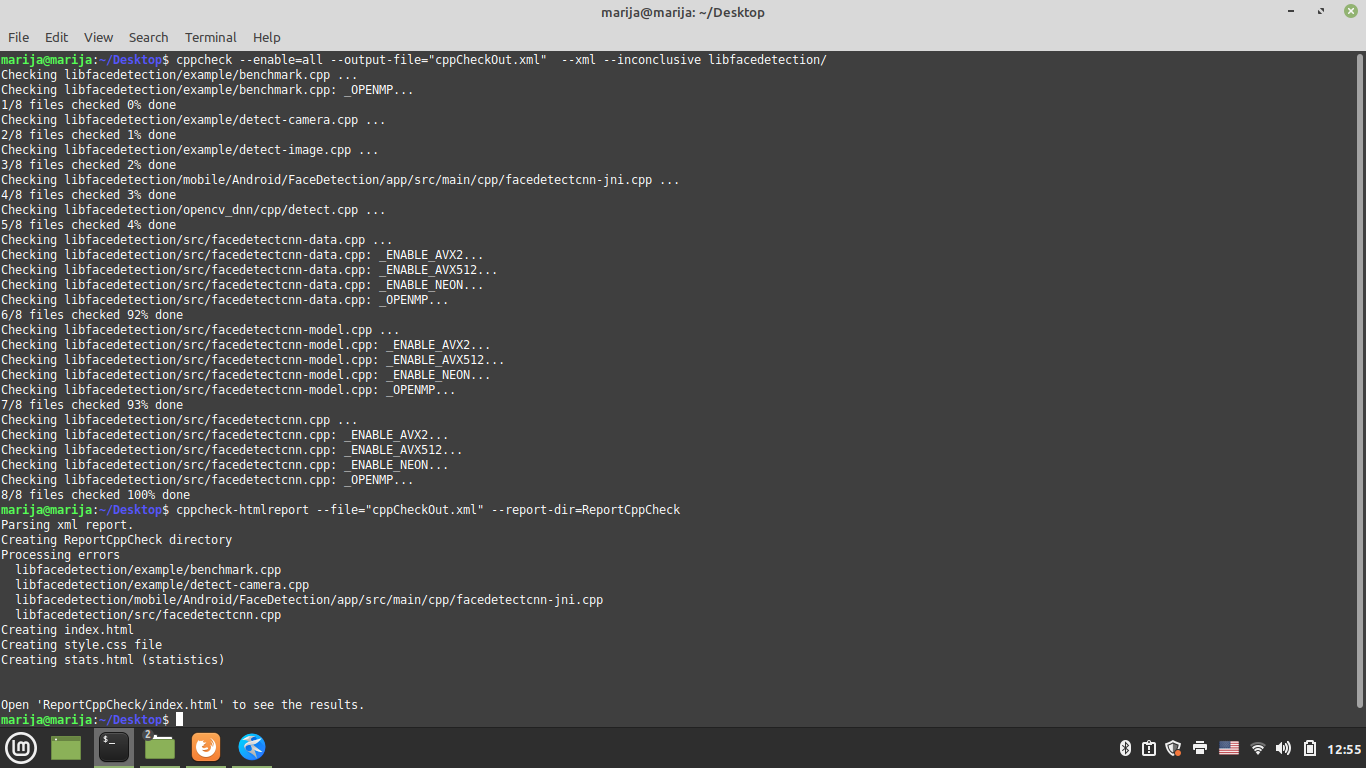
\includegraphics[width=12cm]{img/cppCheckTerminal.png}
    \caption{Poruka o gresh\-ci u $cppCheck$}
    \label{msg:cppcheck}
\end{figure}
%----------------------------------------------------------------%
\paragraph{Rezultati analize:}
Na slici \ref{stats:cppcheck} se nalazi statistika analize.

\begin{figure}[H]
    \centering
    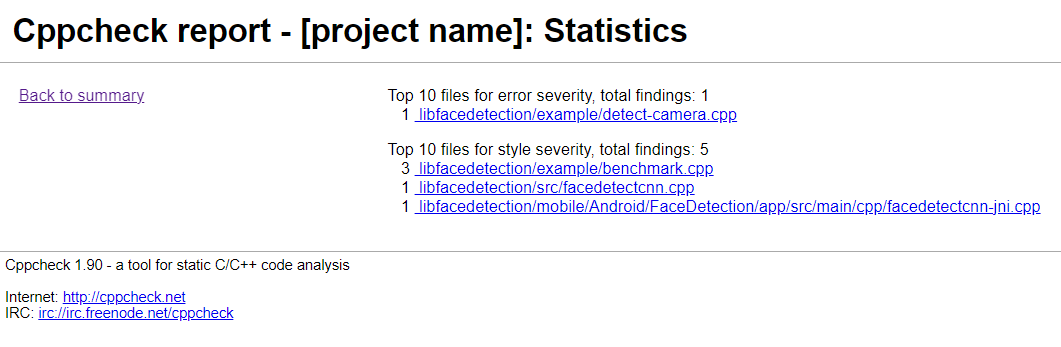
\includegraphics[width=12cm]{img/cppCheckStats.png}
    \caption{Statistika analize alata $cppcheck$}
    \label{stats:cppcheck}
\end{figure}
Na osnovu statistike vidimo da je pronadjena jedna poruka tipa \textit{greshka}, i 5 poruka tipa \textit{stil}.

Detaljnije o porukama se mozhe videti na slici \ref{html:cppcheck}.
\begin{figure}[H]
    \centering
    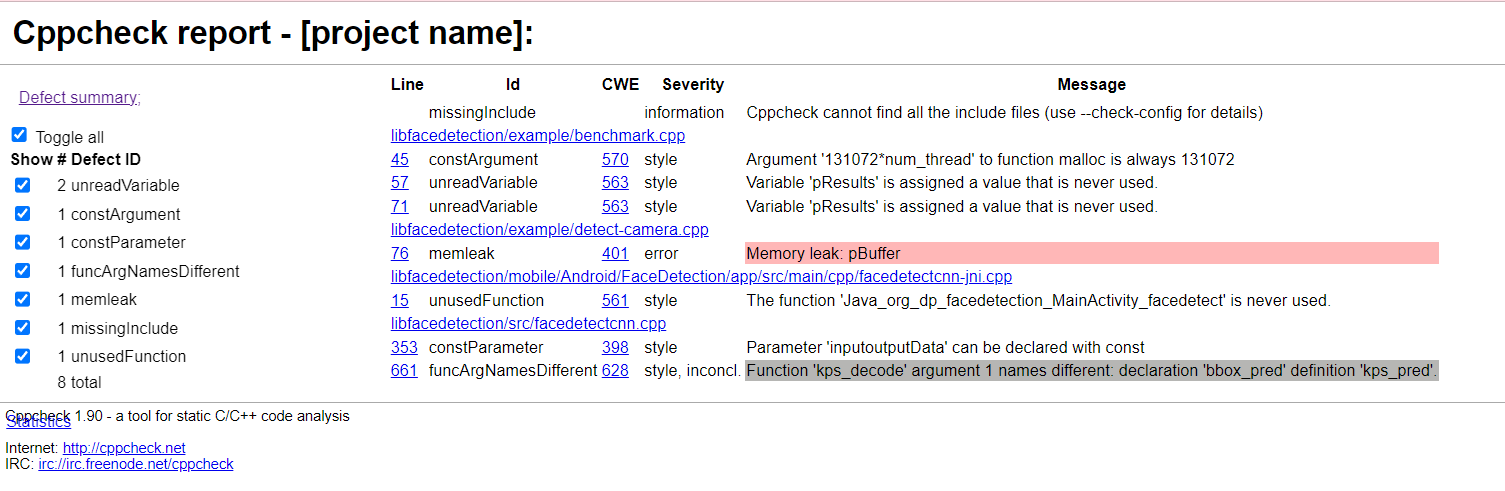
\includegraphics[width=12cm]{img/cppChechHtmlReport.png}
    \caption{Izveshtaj alata $cppcheck$}
    \label{html:cppcheck}
\end{figure}

Greshka se nalazi u 76 liniji u fajlu $detect-camera.cpp$. Deo koda koji izaziva gresku je dat u nastavku:
\fontencoding{T1}\selectfont

\inputminted[frame=lines,
framesep=2mm,
baselinestretch=1.2,
bgcolor=LightGray,
fontsize=\footnotesize,
firstline=55,
lastline=77,
linenos
]{cpp}{detect-camera.cpp}

\fontencoding{OT2}\selectfont
Dakle, memorija koje je alocirana u liniji 59 se ne oslobadja pre prekida izvrshavanja programa, ukoliko je $VideoCapture$ neuspeshno otvoren.

Pored toga su prijavljena upozrorenja za nekorishcene promenljive i funkcije. Detaljan izveshtaj se mozhe pronac1i u okviru repozitorijuma za analizu projekta, u okviru foldera $CppCheckReport.$ U navedenom repozitorijumu je za svaki fajl u kome je alat pronashao neki problem napravljen $html$ izveshtaj sa obelezhenim mestima sa pronadjenim problemima.


\fontencoding{OT2}\selectfont
Takodje, moguc1e je pokretanje alata u okviru razvojnog okrizhenja $QtCreator.$ Poshto nije 
\fontencoding{T1}\selectfont
\textbf{Help->About Plugins -> Code Analyzer}.
\fontencoding{OT2}\selectfont
Izabrati $Cppcheck$. Nakon toga 
je neophodno restartovanje okruzhenje.

Nakon toga: 
\fontencoding{T1}\selectfont
\textbf{Analyze -> Cppcheck}
\fontencoding{OT2}\selectfont
nakon chega se otvara prozor prikazan na slici \ref{qt:cppcheck}.

\begin{figure}[H]
    \centering
    \includegraphics[width=10cm]{img/CppCheckQt.png}
    \caption{Pokretanje alata u okviru $QtCreatora$}
    \label{qt:cppcheck}
\end{figure}

Selektovanjem polja $inconclusive$ $errors$ se prijavljuju i lazhna upozorenja ($false$ $positive$). 

\section{Pokretanje skripti}
\fontencoding{T1}\selectfont

\begin{minted}{shell-session}
git clone ...
\end{minted}

\subsection*{$CppCheck$}
\begin{minted}{shell-session}
cd 2023....
cd libfacedetection
git submodule update
cd ../CppCheckReport
bash runCppCheck.sh
\end{minted}
\fontencoding{OT2}\selectfont

\bibliographystyle{plain}
\fontencoding{T1}\selectfont
\bibliography{literatura}

\end{document}
